\documentclass[11pt]{article}

\usepackage{graphicx}
\usepackage{wrapfig}
\usepackage{url}
\usepackage{wrapfig}
\usepackage{color}
\usepackage{marvosym}
\usepackage{enumerate}
\usepackage{subfigure}
\usepackage{tikz}
\usepackage{amsmath}
\usepackage{amssymb}
\usepackage{hyperref} 


\oddsidemargin 0mm
\evensidemargin 5mm
\topmargin -20mm
\textheight 240mm
\textwidth 160mm

\newcommand{\vwi}{{\bf w}_i}

\pagestyle{myheadings} 
\markboth{}{Law of Large Graphs}

\title{Law of Large Graphs}
\author{}
\date{}

\begin{document}
\large
\maketitle
\thispagestyle{headings}

\vspace{-.5in}

\section{Introduction}
Here we are looking at the scenario where we have M adjacency matrices, $A_m$, that are sampled from the same statistical model, each with N vertices, with known vertex correspondences.  We are looking at methods that estimate the edge probability matrix P, which includes the naive case of averaging over the M adjacency matrices, $\bar{A}$, as well as spectral approaches, where we are taking the spectral decomposition of $\bar{A}$.
\section{Model and Notation}
\paragraph{1. Stochastic Block Model}
We are considering a \textit{k}-dimensional Stochastic Block Model (SBM) for an N vertex undirected hollow graph with block probability matrix \textbf{B} and a block membership probability vector $\rho$.\\\\
We will often consider a generalized Stochastic Block Model with latent positions distributed according to a mixture of Dirichlet random variables using parameter $r \in [0,  \infty )$,  where an exact SBM is obtained at $r = \infty$, and $r = 0$ leads to a uniform distribution.\\\\
Given the model parameters the edge probability matrix $P \in [0,1]^{NxN}$ is calculated.  M instances of adjacency matrices with known vertex correspondence are sampled with $A_{ij} \sim Bern(P_{ij})$.  With these $A_m$ for m in $1,...,M,$ then $\bar{A} = \frac{1}{M}\sum\limits_{m = 1}^M A_m$.

\paragraph{2. Spectral Embedding and Clustering} Since P is positive and semidefinite with rank at most \textit{k}, P has a spectral decomposition $P = VSV^T$, where $V \in R^{Nxk}$ has orthonormal columns and S is diagonal with decreasing entries.  X is then $VS^{1/2}$, and $P=XX^T$.  Let $\bar{A} = U_{\bar{A}}S_{\bar{A}}U_{\bar{A}}^T$ be the full rank decomposition of $\bar{A}$.  Then our estimate of X (subject to a rotation) is $\hat{X} = \hat{V}\hat{S}^{1/2}$, where $\hat{S} \in R^{dxd}$ is the diagonal matrix with the \textit{d} largest magnitude eigenvalues of $\bar{A}$ and $\hat{V} \in R^{Nxk}$ is the matrix with orthonormal columns of the corresponding eigenvectors.

Further, the rows $\hat{X}$ can be clustered into \textit{k} clusters by minimizing mean squared error.  By taking each row to be the mean of it's respective cluster, we get $\hat{X}_c$.

\paragraph{3. Mean Estimators}  We are looking at three estimators for the mean:
\begin{enumerate}
\item $\bar{A}$, taking the average over M samples.
\item $\hat{P} = \hat{X}\hat{X}^T$
\item $\hat{P_c} = \hat{X_c}\hat{X_c}^T$
\end{enumerate}
\section{Experimental Results} Testing began by comparing, through mean squared error from P, these mean estimators under four cases, while varying the value of r, the Dirichlet parameter:
\begin{enumerate}
	\item M = 1, N = 10
	\item M = 100, N = 10
	\item M = 1, N = 100
	\item M = 100, N = 100
\end{enumerate}

In general the rank-k approximation is the optimal estimator for the p matrix. however as the variance of probabilities between classes decreases, a lower rank may perform better for the M/N $\rightarrow$ 0 case (M=1, N=100).  Clustering performs best as r $\rightarrow \infty$.  As r$\rightarrow$ 0, the non-clustered spectral embedding performs better, however this effect happens slower as M/N $\rightarrow$ 0.  The naive approach is the optimal estimator, compared to the low rank approximations, in the case where M/N is large (M=100, N=10 case) and r is small.
\\\\
For the following experiments:
\begin{equation*}
B = \begin{bmatrix}
.42 & .2 \\
.2 & .7 
\end{bmatrix}
,\qquad \rho = \begin{bmatrix}
.5 & .5
\end{bmatrix}
\end{equation*}
We are showing violin plots of the mean squared error of our estimator compared to the true P matrix for a specified r value.  For spectral embedding we test several rank-d approximations.  Below, an example of a P matrix is shown as well as the distribution of the dirichlet random variable latent space. 
\newpage
\begin{figure}[!htb]
	\centering
	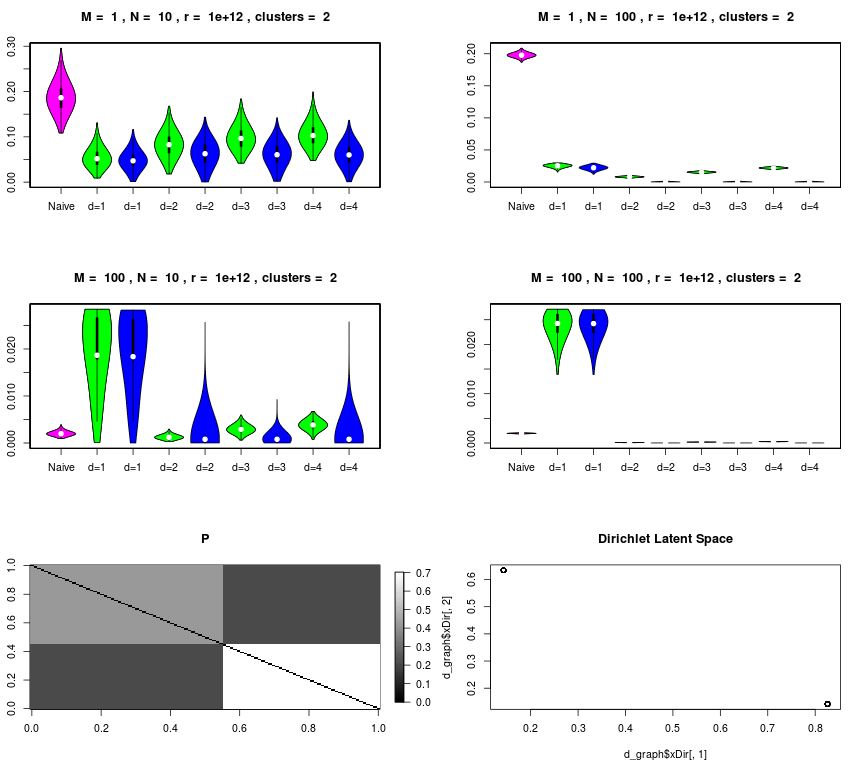
\includegraphics[width=18cm]{Capture1.jpg}
	\caption{For high r, we approach an exact SBM. Here we see that embedding (tpyically rank-k) performs better than the naive approach in all cases. For the rank-k approximation in N=100, and M=1, M=100, clustering leads to decreased error (compared to non-clustering spectral embedding) in both cases.}
	\label{fig:plot1}
\end{figure}
\newpage
\begin{figure}[!htb]
	\centering
	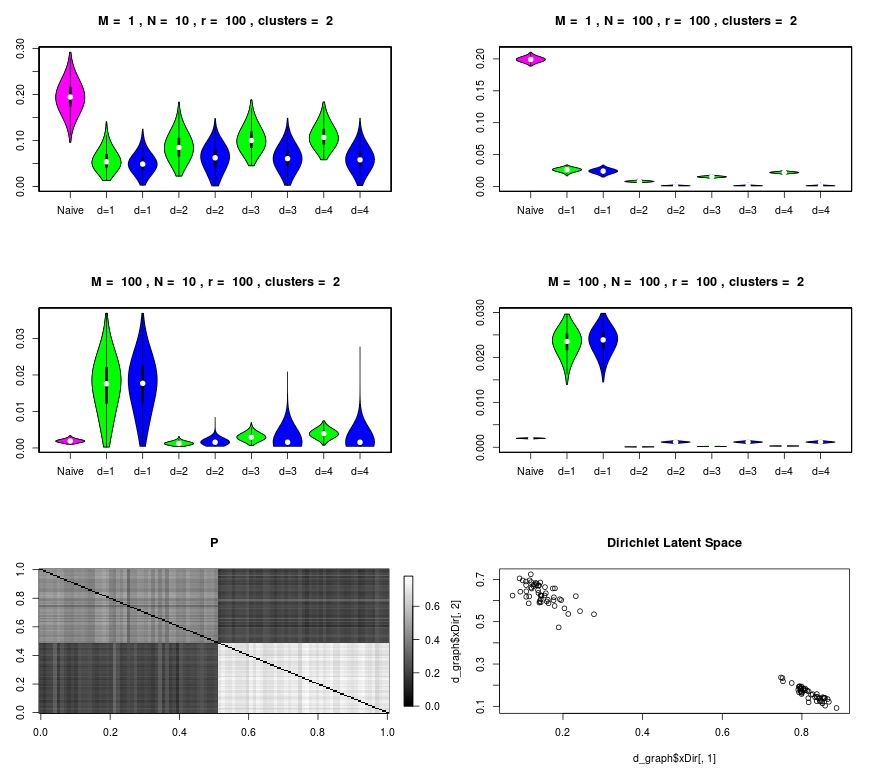
\includegraphics[width=18cm]{Capture2.jpg}
	\caption{As r decreases to 100, we see that in the N=100, M=100 case, that clustering leads to increased error (compared to non-clustered spectral embedding), while it still shows decreased error for M=1. N=100}
	\label{fig:plot1}
\end{figure}
\newpage
\begin{figure}[!htb]
	\centering
	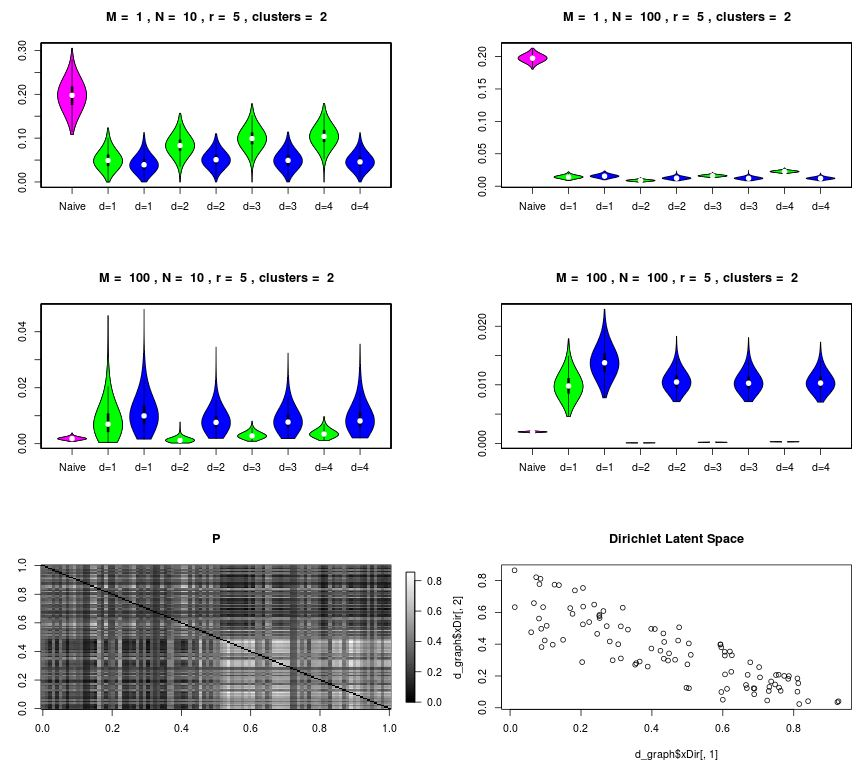
\includegraphics[width=18cm]{Capture3.jpg}
	\caption{As r decreases to 5, we see that clustering leads to increased error (compared to non-clustered spectral embedding) for both N=100 cases for at least the rank $\leq k$ approximations}
	\label{fig:plot1}
\end{figure}
\newpage
Now we switch to \begin{equation*}
B = \begin{bmatrix}
.42 & .42 \\
.42 & .5 
\end{bmatrix}
,\qquad \rho = \begin{bmatrix}
.5 & .5
\end{bmatrix}
\end{equation*}
\begin{figure}[!htb]
	\centering
	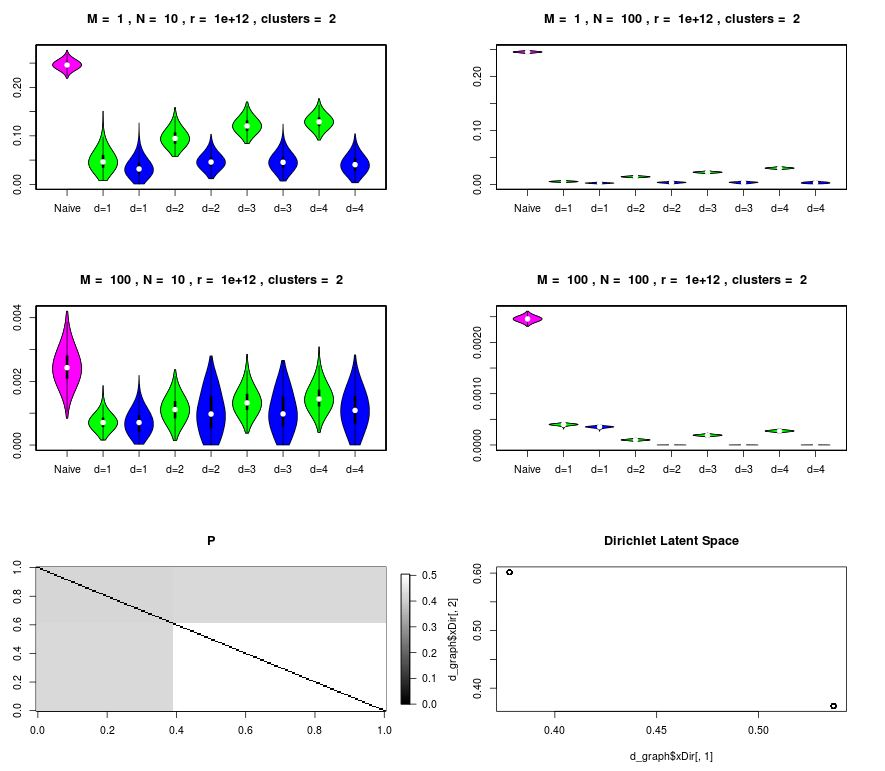
\includegraphics[width=18cm]{Capture4.jpg}
	\caption{As the variance between block probabilities decreases, rank $< k$ approximations show lower error in the $M/N \rightarrow 0$ case}
	\label{fig:plot1}
\end{figure}
\newpage
\section{Theory Questions}
\paragraph{} Here are some of the theoretical questions we would like to look at for this setting. Most of the thoughts were extending previous work to $M > 1$. 
\\\\
How the variance of the Latent Positions  of $\bar{A}$ is affected as a function of M.
\\\\
We would also want to try to get bounds for $|| P - \hat{P}|| = || XX' - \hat{X}\hat{X}^T||$  and $|| P - \bar{A} ||$ dependent on M.  For the case of M = 1,  similar results have been shown in some of the previous papers.  i.e. $|| P - A ||$ and $|| X - \hat{X}||$ (This we'd need to extend to $XX^T$).  Again need to extend it to $M>1$.

\begin{figure}[!htb]
	\centering
	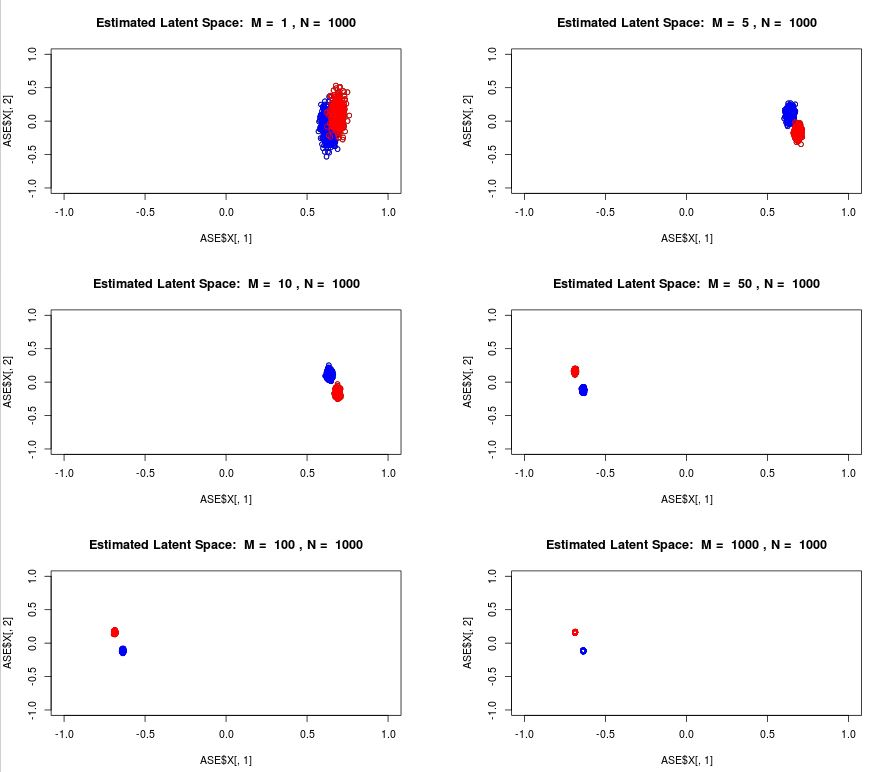
\includegraphics[width=18cm]{Capture5.jpg}
	\caption{We can see that as we increase M, the variance of the latent space for $\bar{A}$ decreases}
	\label{fig:plot1}
\end{figure}
\end{document}
